\documentclass{article}
\usepackage[utf8]{inputenc}
\usepackage[spanish]{babel}
\usepackage{listings}
\usepackage{graphicx}
\graphicspath{ {/home/mafeta/Imágenes/parcial1}}
\usepackage{cite}

\begin{document}

\begin{titlepage}
    \begin{center}
        \vspace*{1cm}
            
        \Huge
        \textbf{Análisis y Diseño Parcial 1}
            
        \vspace{0.5cm}
        \LARGE
        Sistema de encriptación 
            
        \vspace{5cm}
            
        \textbf{Maria Fernanda Tasco ALquichire}
            
        \vfill
            
        \vspace{0.8cm}
            
        \Large
        Despartamento de Ingeniería Electrónica y Telecomunicaciones\\
        Universidad de Antioquia\\
        Medellín\\
        Febrero de 2022
            
    \end{center}
\end{titlepage}

\tableofcontents
\newpage

\section{Objetivos}\label{intro1}
\subsection{generales}
resumen - abstrac
\subsection{Especificos}
introducion

\section{Sección introductoria}\label{intro2}
\subsection{Resumen}
resumen - abstrac
\subsection{Introdución}
introducion


\section{Marco Teorico} \label{investigación}
Esta sección es para agregar toda la información correspondiente con código, citas, etc.

\subsection{Terminología / preguntas en la investigación}
\subsubsection*{¿Qué es, para qué sirve y cómo se usa la señal de reloj?}
Una \textbf{Señal de Reloj} \cite{senal_reloj} es una señal usada para coordinar las acciones de 2 o más circuitos o sistemas. Oscila entre estado alto y bajo en forma de señal cuadrada.
\\[0.2cm]
En este caso se usará un primer reloj para sincronizar los datos que estarán en la primera parte de registro de desplazamiento, es decir autorizar la entrada en serie de cada bit. Un segundo reloj para sincronizar el registro de almacenamiento que autoriza el paso de los datos que van a estar en la salida (estos relojes están implementados dentro de CI 74HC595). Una breve representación la podemos ver en la figura 1 y 2.

\begin{figure}[!ht]
\caption{74HC595 con los mismo bits en el \textbf{registro} \cite{registro_desplazamiento_almacenamiento} de desplazamiento y almacenamiento }
\centering
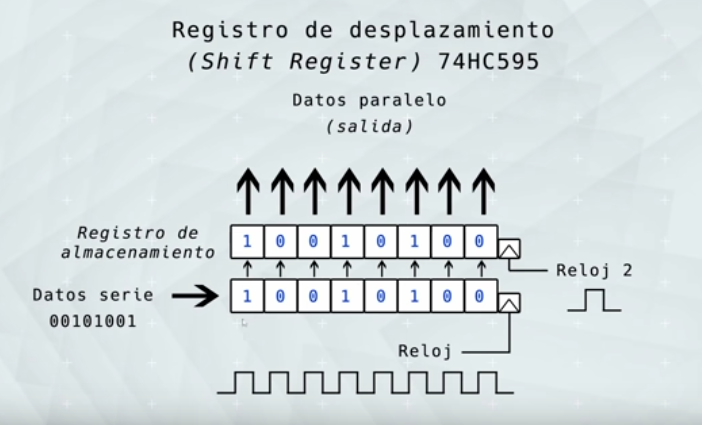
\includegraphics[width=0.5\textwidth]{registro_desplazamiento1.png}
\end{figure}

\begin{figure}[!ht]
\caption{74HC595 con un nuevo byte en el \textbf{registro} \cite{registro_desplazamiento_almacenamiento} de desplazamiento y el byte anterior en el de almacenamiento }
\centering
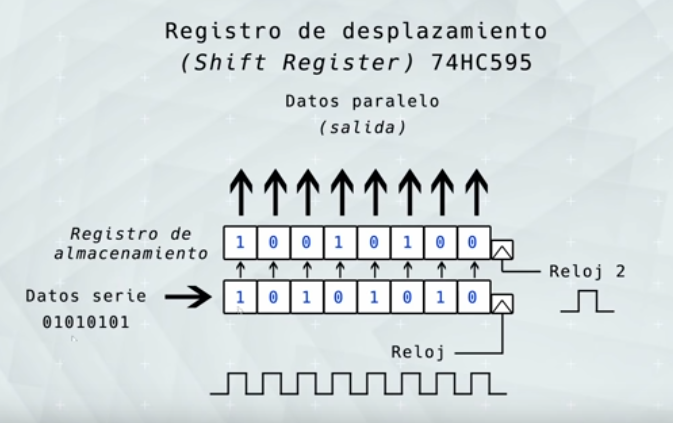
\includegraphics[width=0.5\textwidth]{registro_desplazamiento2.png}
\end{figure}

\subsubsection*{¿74HC595?}
El circuito integrado 74HC595 es un \textbf{registro de desplazamiento} \cite{74HC595Informacion}  que cuenta con entrada en serie y salida en paralelo de 8 bits. Lo que quiere decir es que en este \textbf{tipo de registros} \cite{tipo_de_registros} con salida en paralelo se dispone de la salida de cada \textbf{flip-flop o biestable} \cite{flip-flop_o_biestable} que nos servirá para memorizar la información a la que antes se hacía referencia por lo que una vez almacenados los datos cada bits se representa en su respectiva salida.
\\[0.2cm]
La utilidad que puede darle este elemento a la solución
del problema es que con el \textbf{desplazamiento} \cite{74hc595_como_funciona} de datos y dependiendo del sistema de desencriptación, yo voy a tener en la salida que es paralela el bit que voy a comparar dado el caso, mientras que se van ingresando otros bits, y hacer esto de manera sincronica ya que con la ayuda de los relojs ayuda a que las salidas no se vea afectada con la entrada, así finalmente ganando eficiencia y agilidad.
\\[0.2cm]
\textbf{Otra utilidad} \cite{registro_desplazamiento_almacenamiento} que tiene este CI en especial es el RCLK (Registro de reloj/Latch) Cuando este en BAJO (LOW), el contenido del registro de desplazamiento (los 8 bits) se copia en el registro de almacenamiento; que finalmente se muestra en la salida. Eso permite que mientras se realiza este proceso se puedan ir ingresando datos en serie usando el SRCLR (Shift Register Clear) que reinicia todo el registro de desplazamiento, haciendo que todos sus bits sean 0, cuando este esta en LOW y así dando paso a que el SRCLK (Shift Register Clock) que registra el cambio y desplaza los bits en el registro de desplazamiento, cuando este esta en HIGH. Una pequeña representación en la figura 3.

\begin{figure}[!ht]
\caption{74HC595 con el \textbf{registro} \cite{registro_desplazamiento_almacenamiento} de desplazamiento y almacenamiento con los pines más importantes y los de salida}
\centering
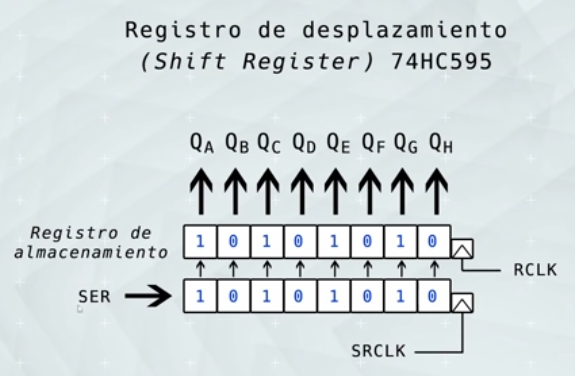
\includegraphics[width=0.5\textwidth]{registro_desplazamiento_pines.png}
\end{figure}

Se puede ver la implementación de este CI con pulsadores / switches y con arduino en la sección de marco experimental.

\subsubsection*{¿Qué variable usar para un arreglo de números enteros de 1byte?}
Inicialmente en el programa de Qt se hará uso de la variable unsigned char (es una variable que almacena 8bits sin signo, desde 0-255) que aunque no pueda imprimir caracteres que no son imprimibles, solo se usará para que al leer el archivo de texto encriptado guarde la información allí. En arduino se hará el uso del tipo de variable byte (es una variable que almacena 8bits sin signo, desde 0-255). Así las dos variables tienen el mismo tamaño lo cuál ayuda a que en el paso de información no haya algún problema.

\subsubsection*{¿Cómo se pueden conectar dos arduinos,y con qué fin?}
Se usan los conceptos de maestro y esclavo. El arduino esclavo en este caso será el que cumplirá la función de sistema de recepción y el arduino maestro es el que obtendrá los datos iniciales que serán procesados para obtener el mensaje real que se le pasará al arduino esclavo para que al final lo muestre por medio de una pantalla lcd.
\\[0.2cm]
El objetivo de esta parte es \textbf{cómo enviar bits} \cite{conexion_dos_arduinos} desde uno y ser recibidos por el otro
de forma exitosa.
Para empezar sus tierras/GND deben ser la misma para tener el mismo potencial electrico y no hayan complicaciones luego. Se usa la libreria <Wire.h> ya que tiene funciones para la comunicación. Esto se puede en la figura 4.

\begin{figure}[!ht]
\caption{Conexión entre  \textbf{arduinos} \cite{conexion_dos_arduinos} usando la libreria Wire.h}
\centering
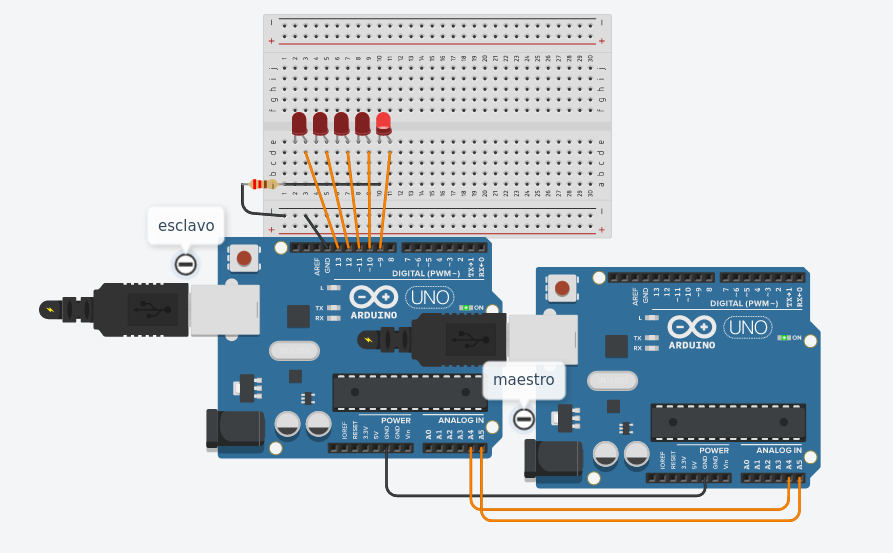
\includegraphics[width=0.5\textwidth]{conexion_arduinos.png}
\end{figure}

\subsection{Investgación soluciuones propuestas}
aun no he investigado nada


\section{Marco Expremiental} \label{practica}
\subsection*{74HC595 Ejemplo de uso con pulsadores / switches}
Para esta primera implementación de ejemplo se probará el 74HC595 con un \textbf{pulsador} \cite{74hc595_pulsador} que registra los desplazamientos, otro que registra la salida y el interruptor deslizante como entrada (HIGH-LOW). Se puede ver en la figura 5.

\begin{figure}[!ht]
\caption{Uso 74HC595 con pulsadores en \textbf{tinkercad} \cite{ejem_74HC595_pulsadores}}
\centering
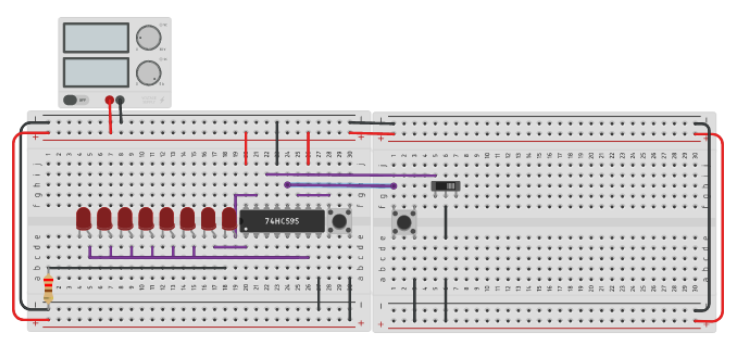
\includegraphics[width=0.5\textwidth]{ejem_75hc595_pulsadores.png}
\end{figure}

Por último se implementó el CI con arduino, en este caso colocando los 3 pines principales (SER: a donde enviar los datos serie, SRCLK: reloj del registro de desplazamiento, RCLK: reloj del registro de almacenamiento) en los pines digitales de arduino, también se hizó uso de la función shiftOut(); de \textbf{arduino} \cite{shiftOut_arduino}  la cual es la función estrella en el registro de desplazamiento ya que recibe 4 parametros (SER,SRCLK,LSBFIRST/MSBFIRST,i) el tercere parametro es para definir el orden de la entrada si desde el primer bit o el segundo, en este caso para que al ingresar y desplazar los bits y al final me quede el byte que se ingreso por medio de la variable i se usará el LSBFIRST. Se puede ver en la figura 6.

\begin{figure}[!ht]
\caption{Uso 74HC595 con arduino en \textbf{tinkercad} \cite{ejem_74hc595_arduino}}
\centering
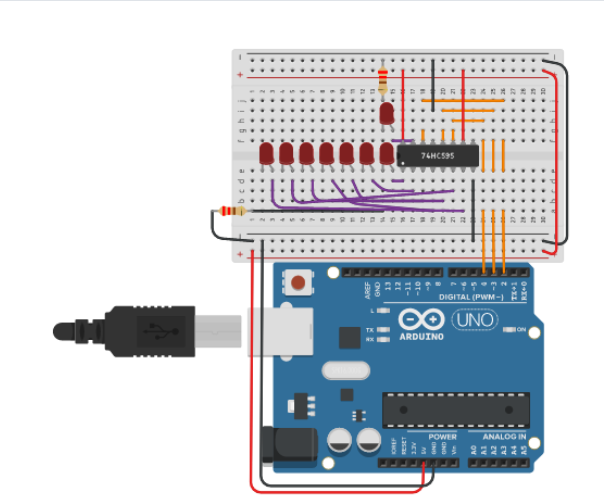
\includegraphics[width=0.5\textwidth]{Ejem_74hc595_arduino.png}
\end{figure}

con esto se concluye que el uso del primer reloj en este CI nos ayuda a sincronizar los datos que van entrando en Serie al 74HC595 y gracias al segundo reloj que tiene implementado este CI nos ayuda a hacer el registro de almacenamiento con un único pulso, permitiendo almacenar los datos que van a la salida mientras que se van ingresando otros datos en el registro de desplazamiento; esto asegura que la salida no se vea afectada mientras que se hace la carga.


\section{Resultados} \label{conclusiones}
Una clave para el desarrollo del algoritmo fue el orden de los pasos, ya que un orden adecuado, omitir algunos pasos o no generar las condiciones necesarias para el buen desarrollo de la solución, podría generar alguna ambigüedad o error.

\section{Conclusiones} \label{conclusiones}
Una clave para el desarrollo del algoritmo fue el orden de los pasos, ya que un orden adecuado, omitir algunos pasos o no generar las condiciones necesarias para el buen desarrollo de la solución, podría generar alguna ambigüedad o error.



(\ref{intro1}),(\label{intro2}), (\label{investigación}), (\label{practica}), (\label{conclusiones}) y (\label{practica})
\bibliographystyle{IEEEtran}
\bibliography{references}

\end{document}

